\documentclass{article}

\usepackage[utf8]{inputenc}
\usepackage{amsthm}
\usepackage{amsmath}    % Extended typesetting of mathematical expression.
\usepackage{amssymb}    % Provides a multitude of mathematical symbols.
\usepackage{mathtools}  % Further extensions of mathematical typesetting.
\usepackage{microtype}  % Small-scale typographic enhancements.
\usepackage{multirow}   % Allows table elements to span several rows.
\usepackage{booktabs}   % Improves the typesettings of tables.
\usepackage{subcaption} % Allows the use of subfigures and enables their referencing.
\usepackage[ruled,linesnumbered]{algorithm2e} % Enables the writing of pseudo code.
\usepackage[tmargin=2cm,rmargin=1in,lmargin=1in,margin=0.85in,bmargin=2cm,footskip=.2in]{geometry}

\usepackage[usenames,dvipsnames,table]{xcolor} % Allows the definition and use of colors. This package has to be included before tikz.
\usepackage{tikz}
\usepackage{multicol}
\usetikzlibrary{calc}
\usepackage{nag}       % Issues warnings when best practices in writing LaTeX documents are violated.
\usepackage{todonotes} % Provides tooltip-like todo notes.
\usepackage{hyperref}  % Enables cross linking in the electronic document version. This package has to be included second to last.
\usepackage[backend = biber, style = ieee]{biblatex}
\usepackage{tcolorbox}

\usepackage{titlesec}
\titleformat{\subsubsection}[runin]{\bfseries}{}{}{}[.]

\usepackage{fancyhdr}
\pagestyle{fancy}
\renewcommand{\headrulewidth}{0.4pt}

\title{Custom Project Proposal - No Kangaroos in Austria}
\author{Florian Schager}

\chead{\textbf{No Kangaroos in Austria}}

\begin{document}


\newenvironment{Figure}
  {\par\medskip\noindent\minipage{\linewidth}}
  {\endminipage\par\medskip}

\definecolor{darkorange}{rgb}{1, 0.549, 0}
\definecolor{turquoise}{rgb}{0.251, 0.879, 0.816}
\tcbset{
    frame code={}
    center title,
    left=0pt,
    right=0pt,
    top=0pt,
    bottom=0pt,
    colback=darkorange!30,
    colframe=white,
    enlarge left by=0mm,
    boxsep=5pt,
    arc=0pt,outer arc=0pt,
    }

\maketitle

In the game GeoGuessr the player is dropped on a random location within Google Streetview
with the goal to determine his location as precisely as possible.
In the simplest case, we are not allowed to move from our starting position,
pan around nor zoom in the initial image.

\begin{figure}[hbt!]
  \centering
    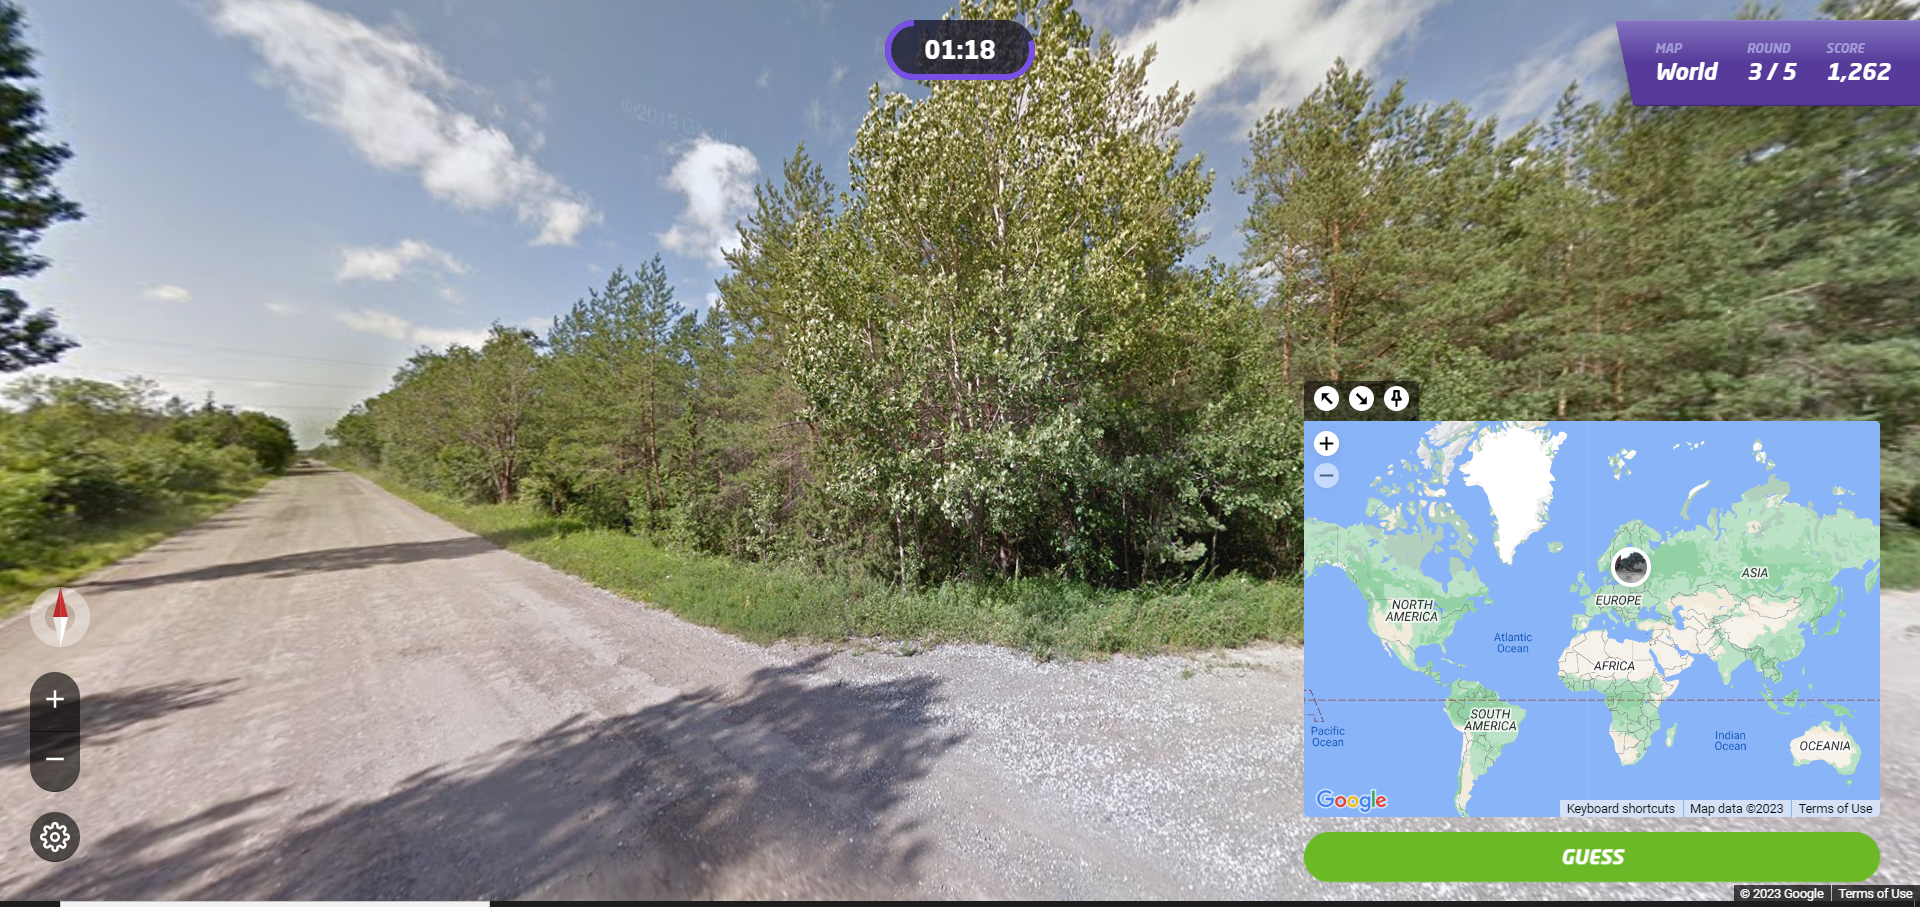
\includegraphics[width = 0.7\linewidth]{example.PNG}
    \caption{Example image from a game of GeoGuessr}
\end{figure}

Hence the goal of this Machine Learning project is to map Street View images to location data.
This setting naturally allows for either regression, where we aim to predict the latitude and longitude of any given image,
or classification, if we ask to classify the images into pre-defined geographic regions, like countries or continents.

To obtain our dataset, we use the osmnx library to create street network graphs for given geographical regions.
This is necessary, because simply sampling geographically uniform points
within a given region is unlikely to return coordinates with street view coverage.
Instead, we can sample our points from these street network graphs, 
which in turn get fed into the Google Street View API.
The API now checks whether there is an available street view image within a fifty meter radius
and if yes, returns one such image.

I want to focus on the classification task, where images are classified into the countries, where they are taken in.
A good starting point would then be to pick two distinct countries, like Austria and Australia
to replace the \texttt{dogs\_vs\_cats} dataset. I would then propose
to more or less keep the individual task of the project as is, except
for the dataset. The only thing I am unsure about in this regard is,
whether it makes sense for this task to use pre-trained weights from
the imagenet dataset, since my particular problem seems to
diverge too much from the idea of the imagenet dataset, where images
are classified by so-called synonym sets.
Hence I think it would make more sense to instead try,
once the models perform well
on the binary classification task, how
well this approach extends to a multinomial classification, where I
increase the number of countries the images are sampled from.




\end{document}
